\chapter{Architecture of OpenBiodiv}
\label{chapter-openbiodiv}

As stated in the Introduction, the goal of the present Ph.D. effort is ``to create an open knowledge-based system of biodiversity information extracted from scholarly literature.'' Biodiversity data is quite heterogeneous and comes from many sources; for example, there is taxonomic data (data about the names and descriptions of species), bio-geographic data (data about occurrences of orgamisms at specific locations), genomic data (data about the genetic makeup of species) and so on. For a detailed domain conceptualization including a full discussion of the types of biodiversity data, please refer later to Chapter~\ref{chapter-ontology}. Due to this heterogeneity and in order to ensure the feasibility of the project as a Ph.D. thesis, the OpenBiodiv system that was developed is focused primarily on creating the models and infrastructure needed for processing scholarly publications of biological systematics and taxonomy. 

As per the publication \cite{noauthor_open_2014}, the system ought to meet criteria such as providing ``a consistent biodiversity information space,'' ``new formats to support novel and diverse uses,'' ``linkages with other resources,'' ``accreditation for researcher's work,'' and others. Deliberations about the system were published in in the pro-iBiosphere final report (\cite{soraya_sierra_coordination_2014}). However, the language of the report is high-level and does not provide a formal specification for the system but rather a set of recommendations on the features and implementation of the system. For this reason, at the onset of the project in attempt for formalize the problem we published the specification and design of OpenBiodiv as Ph.D. project plan (\cite{senderov_open_2016}).

During the iterative process of agile software development, we refined and extended the design and specification informed by the implementation process. This chapter should serve, therefore, as an updated version the Ph.D. project plan and as the current specification and design blueprint for the OpenBiodiv system; subsequent chapters contain discussions of the implementation of particular components of the system.

\section{What is OpenBiodiv?}

The understanding of OpenBiodiv as a knowledge-based system can thus be summarized as follows: OpenBiodiv is a  database of interconnected biodiversity information together with a logic and application layers allowing users to not only query the data but also discover additional facts of relevance implied by the data. The primary sources of information in OpenBiodiv are the journals of the academic publisher Pensoft, the taxonomic treatments\footnote{For a discussion of what a taxonomic treatment is, please refer to the subsequent Chapter~\ref{chapter-ontology}} of Plazi, and the taxonomic backbone of GBIF. In Chapter~\ref{chapter-lod} we explore in detail the data sources and their data models.

The research problem of OpenBiodiv's architecture can postulated as designing an open access RDF semantic graph database, incorporating information stored in Pensoft, Plazi, and GBIF, and allowing the user of the system to ask complicated queries. 

As a blueprint for the type queries in the domain of biodiversity science that should be answerable with the help of the system, we have looked at the list compiled in \cite{pro-ibiosphere_competency_2013}. Examples include: "Is X a valid taxonomic name?" ``What are related names to a given name?'' ``Which authors have published about a given taxon?''

In this chapter we break up OpenBiodiv into components that will be treated in detail in subsequent chapters. We describe how these components inter-operate in order to former the OpenBiodiv knowledge-based system.

OpenBiodiv consists of (1) a semantic graph database, (2) a code base, and (3) a front-end in the form of a web-portal facilitating the access to the underlying knowledge base (Fig.~\ref{fig:openbiodiv-components}). OpenBiodiv enables the flow of information between international repositories for biodiversity data to Biodiversity Data Journal (BDJ) and other journals that use the ARPHA-BioDiv toolkit (\cite{penev_arpha-biodiv:_2017}). As a second step, knowledge is extracted from such journals taking advantage of the TaxPub Document Type Definition (DTD)\footnote{We will take the liberty and refer to TaxPub as an XML schema in the rest of the chapter.} introduced by \cite{catapano_taxpub:_2010}. Example journals include ZooKeys, Biodiversity Data Journal (BDJ), PhytoKeys, MycoKeys, and so on\footnote{The journals can be accessed under \url{https://pensoft.net/browse_journals}.}. At the same time, knowledge is extracted from Plazi TreatmentBank, an archive of legacy biodiversity literature published containing over 200 thousand treatments\footnote{A treatment is a special section in a biological publication describing and discussion a species or a higher taxon. TreatmentBank is accessible under \url{https://pensoft.net/browse_journals}.} and updated every day. Last but not least, these sources are interlinked via GBIF's taxonomic backbone (\cite{gbif_secretariat_gbif_2017}). The extracted knowledge is then stored in a semantic graph database (Fig.~\ref{fig:openbiodiv-sources}).

\begin{figure}
\centering
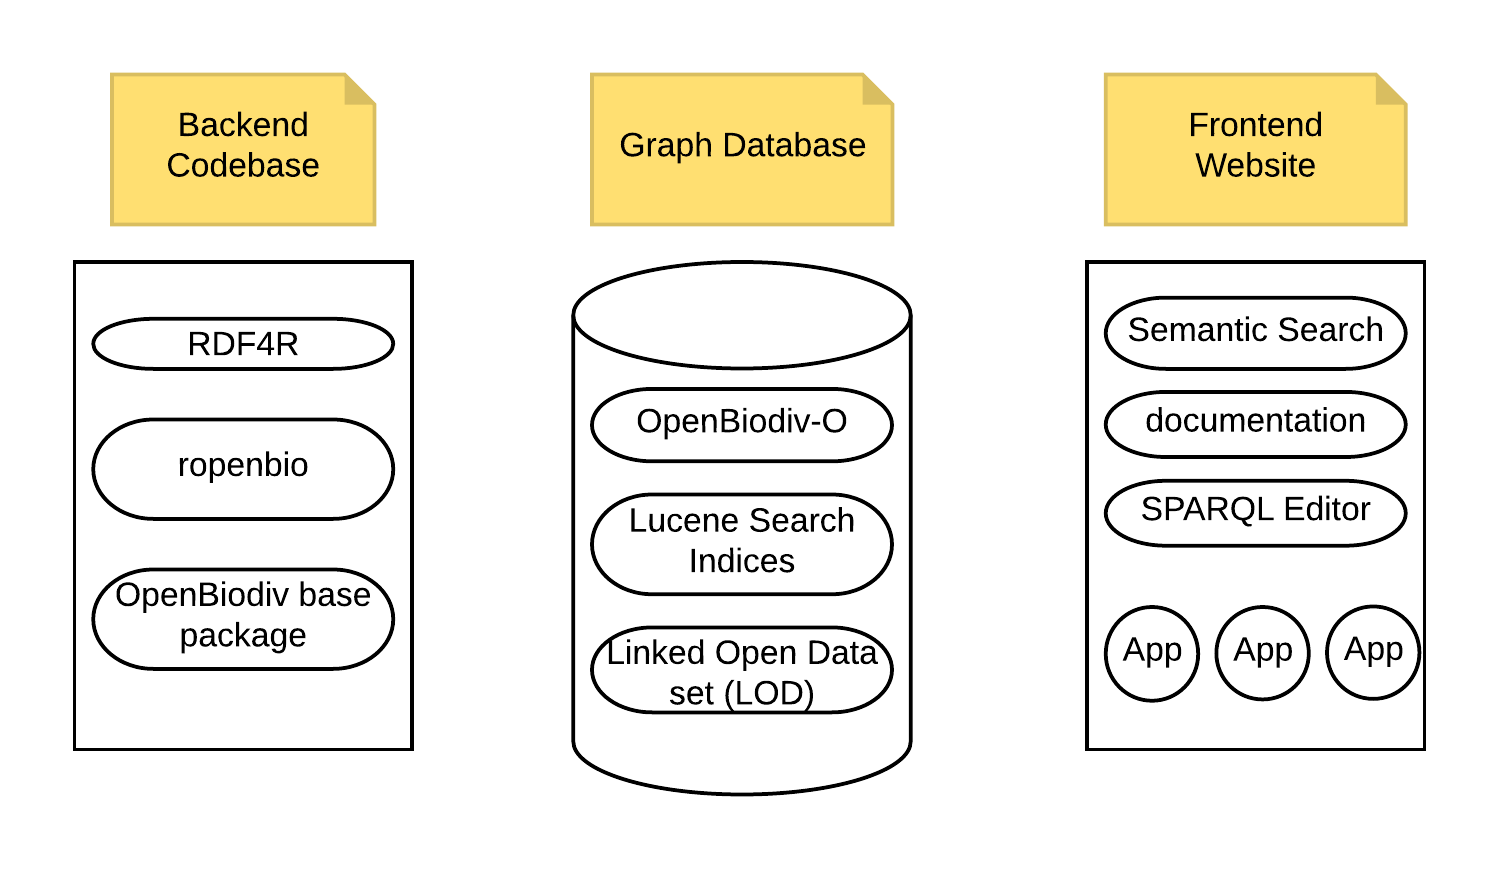
\includegraphics[width=\textwidth]{Figures/components-openbiodiv}
\decoRule
\caption[OpenBiodiv Components]{The components of OpenBiodiv.}
\label{fig:openbiodiv-components}
\end{figure}

\begin{figure}
\centering
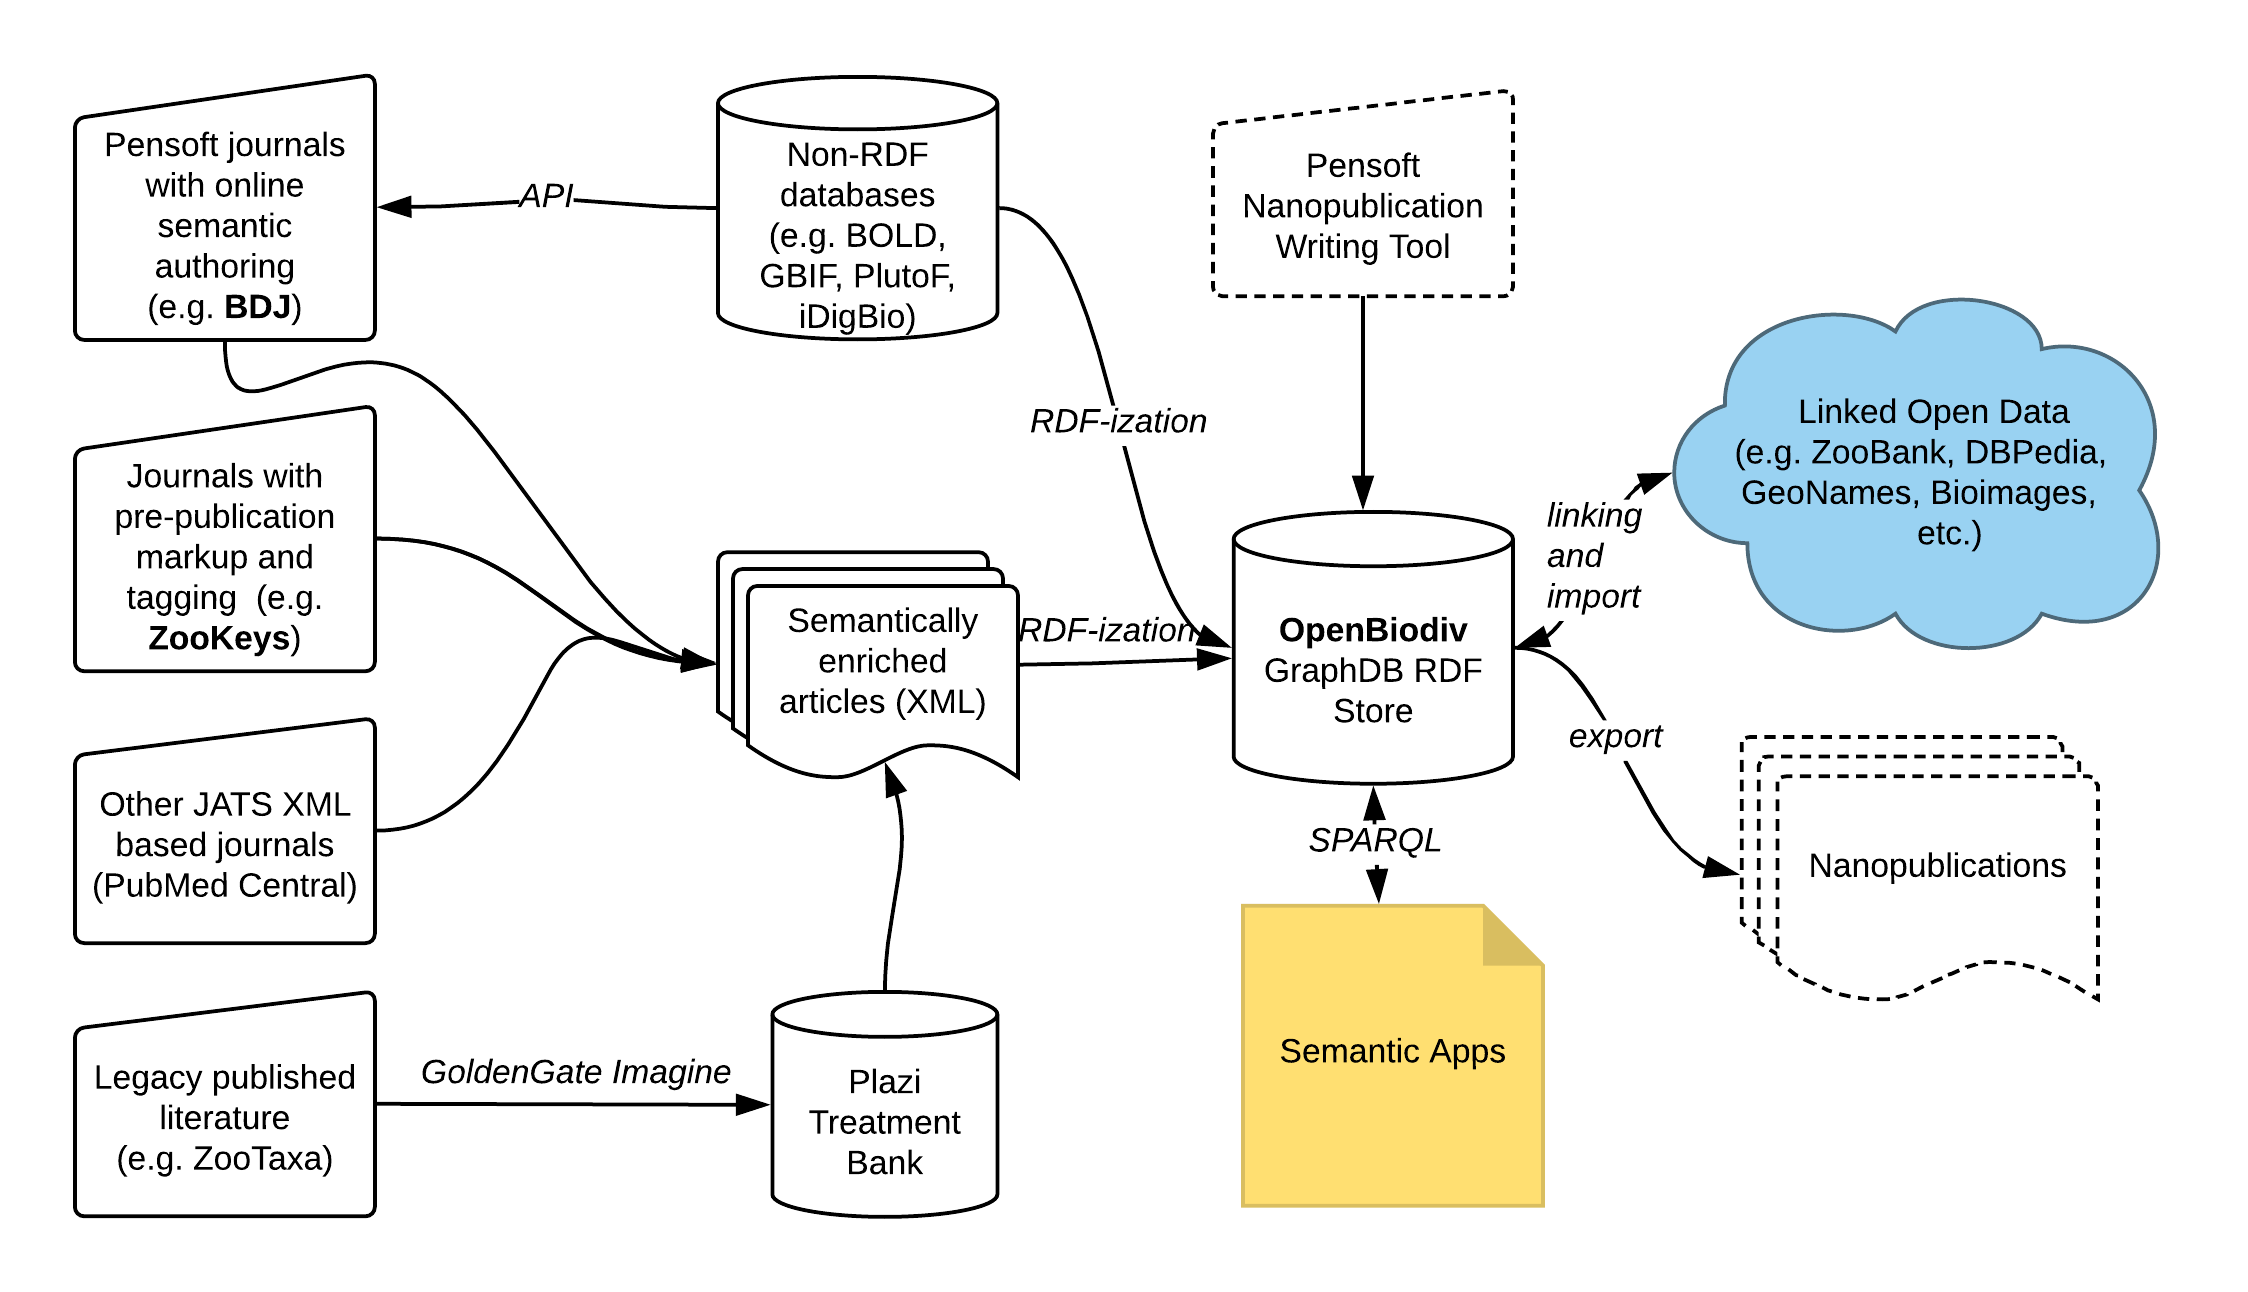
\includegraphics[width=\textwidth]{Figures/openbiodiv-sources}
\decoRule
\caption[OpenBiodiv Components]{Flow of information in the biodiversity data space until it reaches the OpenBiodiv semantic database. Dashed lines are components that have not been implemented yet.
}
\label{fig:openbiodiv-sources}
\end{figure}

\section{Semantic Graph Database}

A primary output of the OpenBiodiv effort is the creation of a semantic database based on knowledge extracted from the archives of Pensoft and Plazi and GBIF's taxonomic backbone and accessible under \url{http://graph.openbiodiv.net/}. A discussion of the components of the database follows.

\subsection{OpenBiodiv ontology (OpenBiodiv-O)}

The central result of the OpenBiodiv effort is the creation of a formal domain model of biodiversity publishing, the ontology OpenBiodiv-O (\cite{senderov_openbiodiv_2017}). The source code of the ontology and accompanying documentation can be accessed under \url{https://github.com/vsenderov/openbiodiv-o}. A detailed discussion is presented in Chapter~\ref{chapter-ontology}.

\subsection{OpenBiodiv Linked Open Dataset (OpenBiodiv-LOD)}

Using OpenBiodiv-O and the infrastructure described later in this chapter a dataset incorporating approximately 200 thousand Plazi treatments, five thousand Pensoft articles, as well as GBIF’s taxonomic backbone (over a million names) has been created. The dataset is available online through the workbench of the semantic database \url{http://graph.openbiodiv.net}. It is discussed in detail in Chapter~\ref{chapter-lod}.

\section{Backend}

In order to populate a semantic database it is necessary to create the infrastructure that converts raw data (text, images, data tables, etc.) into a structured semantic format allowing the interlinking of resource identifiers and the answering of complex queries. OpenBiodiv creates new infrastructure and extends existing infrastructure for transforming biodiversity scholarly publications into Resource Description Format (RDF) statements with the help of the components described in this section.

\subsection{RDF4R: R package for working with RDF}

One of the greater technical challenges for OpenBiodiv is the transformation of biodiversity information (e.g. taxonomic names, paper metadata, figures, etc.) stored as semi-structured XML into fully-structured semantic knowledge in the form of RDF. In order to solve this challenge, an R package has been developed that enables the creation, manipulation, and submission and retrieval to and from a semantic database of RDF statements. This package is accessible under an open source license on GitHub under \url{https://github.com/vsenderov/rdf4r}. We describe the package in Chapter~\ref{chapter-rdf4r}.

\subsection{OpenBiodiv Base and ROpenBio}

In combination with the RDF4R package, the code-base is completed by one more R package, \url{ropenbio} and a code-base (OpenBiodiv Base) of scripts and documentation necessary to bootstrap the database. \url{ropenbio} utilizes the RDF4R package to convert semi-structured XML to RDF. It contains the "mappings" necessary for that conversion. It is available under \url{https://github.com/pensoft/ropenbio}. OpenBiodiv Base coordinates the invocation of \url{ropenbio}, contains scripts for the automatic import of new resources, and other housekeeping details. It is available under \url{https://github.com/vsenderov/openbiodiv}. Their usage to generate the OpenBiodiv-LOD is discussed in Chapter~\ref{chapter-lod}.

\subsection{Workflow for converting ecological metadata to a manuscript}  

Ecological Metadata Language (EML) is a popular format for describing ecological datasets (\cite{michener_nongeospatial_1997}). Biodiversity repositories such as GBIF and DataOne make use of this format to describe the datasets that they store. An import pipeline for importing an EML file as a BDJ data paper\footnote{A data paper (\cite{chavan_data_2011}) is a paper in a scholarly (peer-reviewed) journal discussing a scientific dataset.} has been developed as part of OpenBiodiv (\cite{senderov_online_2016}). We describe this workflow in detail in Chapter~\ref{chapter-case-study}. To access the pipeline interactively, go to \url{https://arpha.pensoft.net}, login to the system (registration is free), select ``Start a new manuscript,'' scroll all the way down to ``Import a manuscript,'' and follow the necessary steps to upload an EML and use it as a template for your new manuscript.

\subsection{Workflow for importing specimen data into Biodiversity Data Journal}

One of the important types of biodiversity data is occurrence data---data that documents the presence of a properly taxonomically identified organism at a given location and time. Such data is stored at international repositories such as BOLD, GBIF, PlutoF, and iDigBio. In order to facilitate data publishing, as well as to act as an entry point into OpenBiodiv, a pipeline for importing any occurrence record from these databases into a BDJ taxonomic paper has been developed (\cite{senderov_online_2016}). We describe this workflow in detail in Chapter ~\ref{chapter-case-study}. To access the workflow interactively, go to \url{https://arpha.pensoft.net}, login to the system (registration is free), select "Start a new manuscript," select "Biodiversity Data Journal" as a journal and "Taxonomic Paper" as paper-type and "Create a manuscript." Then, in your new manuscript, expand the "Taxon treatments" section by clicking on the $+$ sign next to it, give a test classification to your treatment (e.g. Animalia), click ``Save'' and you will be presented with a choice of subsections. Click the ``Materials'' section on the left to visualize the workflow. Look at the lower-part of the dialog, where ``You may place multiple ID's...''---this is the part where you select external resource identifiers to be imported to your article.

\section{Frontend}

In addition to providing a searchable database endpoint, a website allowing semantic search and containing specific tasks packaged as apps is being developed (\url{http://openbiodiv.net}). The development of the site extends beyond the scope of the dissertation thesis and is driven by the Pensoft development team. A beta version is already operational Fig.~\ref{fig:website}. A limited discussion is found in Chapter~\ref{webportal}.

\section{IT}

The system is deployed on a Debian GNU+Linux virtual machine. GraphDB runs with a 20 GB heap file and with the RDFS-Plus Optimized rule set\footnote{This is necessitated by the fact that we reached a performance bottleneck the OWL inference. Discussed in Chapter~\ref{chapter-lod}}.  Continuous operation is ensured by the automatic execution of scripts from the \url{run} directory of OpenBiodiv Base.

\begin{figure}
\centering
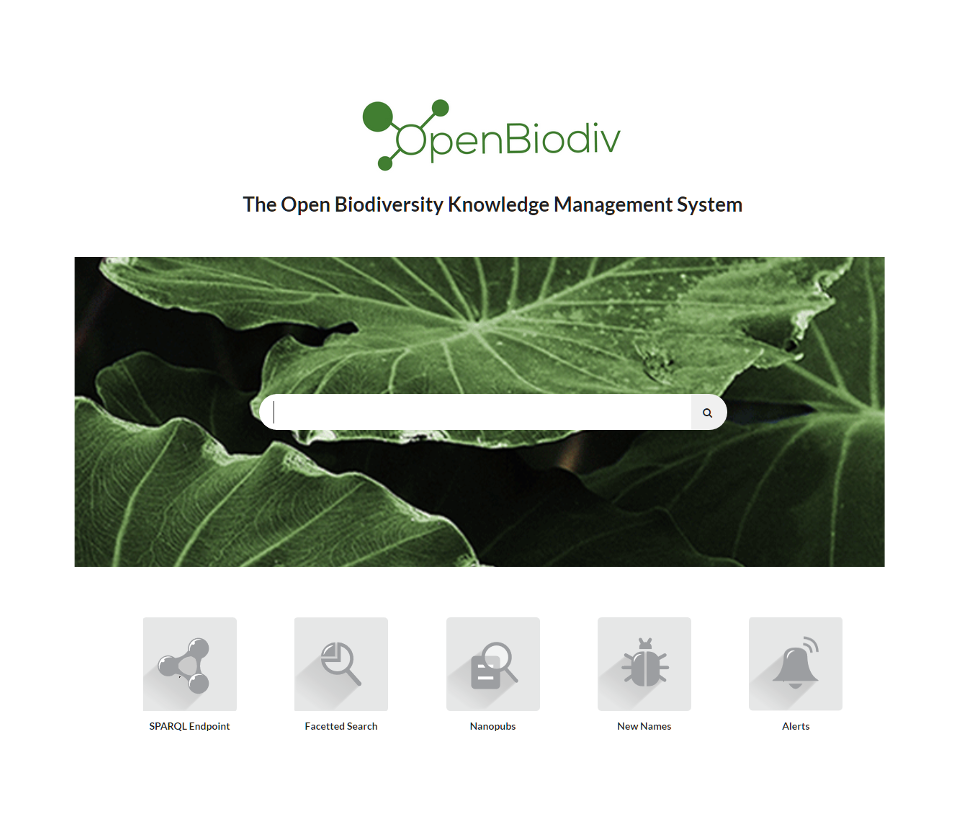
\includegraphics[width=\textwidth]{Figures/openbiodiv-webpage}
\decoRule
\caption[OpenBiodiv Website]{Beta version of the OpenBiodiv website together with sample app icons.}
\label{fig:website}
\end{figure}


